\chapter{Technik}
\label{technik}

Beim Tischfussball ist das Toreschiessen das wichtigste um zu Gewinnen und daher ist das Spiel von Anfängern durch viele schnelle (Direkt-)Schüße geprägt.
Vor allem durch Trichschüsse heben sich erfolgreichere Spieler hervor.
Im Amateur-Bereich kommen meist Pass- und Schuss-Optionen hinzu.
Und im Profi-Bereich werden meist alle Techniken angewandt, vor allem um strategisch eine Partie zu gewinnen. siehe nächstes Kapitel~\ref{taktik}. 
Bei allen Spielniveaus werden verschiedene Defensivtechniken angewandt, um die Offensive des Gegners erfolgreich zu verteidigen.
All diese Techniken sind notwendig für ein kontrolliertes Spiel -- was der eigentlich Trick der Profis ist.

Technik ist die Grundlage eines jeden Sports. 
Das Ziel einer sauberen Technik ist das Kontrollieren des Balles mit den Spielfiguren in unterschiedlichen Spielsituationen:
In der Offensive und bei Ballbesitz gibt es Techniken für das Passen, das Annehmen und das Schießen des Balles (Kapitel \ref{technik:offensive}) -- in der Defensive und bei Nicht-Ballbesitz gibt es Techniken für ein erfolgreiches Stellungsspiel, Bälle zu blocken und zu fangen (Kapitel \ref{technik:defensive}). 
Zunächst in Kapitel \ref{technik:haltung} wird die grundlegende Körper- und Griffhaltung beschrieben, wobei sich vor allem die Griffhaltung und Arm- und Oberkörperbewegung beim Spielen der Techniken verändern kann. 


%%%%%%%%%%%%%%%%%%%%%%%%%%%%%%%%%%%%%%%%%%%%%
\section{Körper- und Griffhaltung}
\label{technik:haltung}





\subsection{Körperhaltung}
\label{technik:haltung:koerper}
Schulterbreiter Stand, nicht auf den Griffen abstützen, sich nicht im weg stehen, vor den Stangen

\subsection{Griffhaltung}
\label{technik:haltung:griffe}



\begin{itemize}
\item Figur zum Ball: Spielen und annehmen
\item Klemmen (Puppenwechsel)
\item Tic-Tac
\end{itemize}

\begin{figure}
    \centering 
        \begin{subfigure}[b]{0.7\textwidth} 
            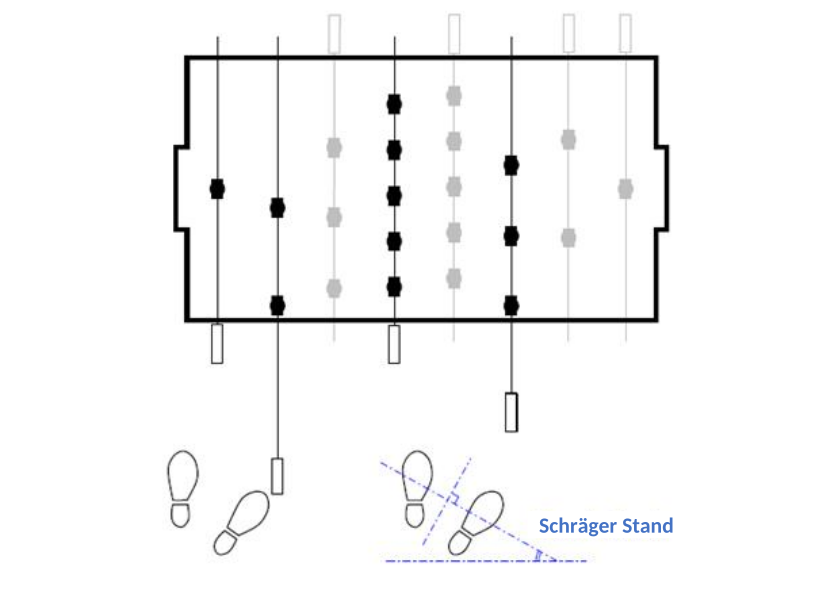
\includegraphics[width=\textwidth]{img/haltung_koerper.png} 
            \caption{Grundlegender Körperstand} 
            \label{fig:haltung:koerper} 
            \vspace{0.5cm}
        \end{subfigure} 
        \begin{subfigure}[b]{0.7\textwidth} 
            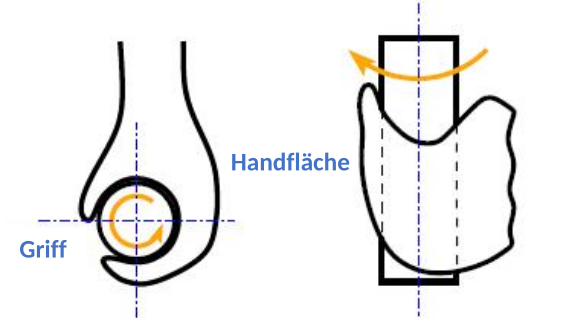
\includegraphics[width=\textwidth]{img/haltung_hand.png} 
            \caption{Grundlegende Handhaltung} 
            \label{fig:haltung:hand} 
        \end{subfigure} 
        \label{fig:haltung} 
        \caption{Die grundlegenden Haltungen [\cite{itsf_basics}]} 
\end{figure}

%%%%%%%%%%%%%%%%%%%%%%%%%%%%%%%%%%%%%%%%%%%%%
\section{Offensive: Passen, Annehmen, Schiessen}
\label{technik:offensive}



GRAFIK: mit Bereichen der Spielfiguren.

Ballgefühl und Dribbling

Grundsätzliches zum Erlernen der \gls{offensive}: ,,Aktion'', altersgerechtes Training,  für Kinder und Jugendliche: weniger statisches Techniktraining, mehr spielerisches Erlernen, siehe Spielformen,


\subsection{Ballführung (auf einer Stange)} 
\label{technik:offensive:eine}

\begin{itemize}
\item Ruhender Ball und Puppenwechsel.
\item Tictac oder Vorne-hinten Klemmen.
\item Auf der 2er-Stange zwischen der 1. und der 2. Puppe.
\item Auf der 3er-Stange zwischen der 1. und der 2. Puppe oder der 2. und der 3.Puppe oder mit der 1. und 3. Puppe.
\item Auf der 5er-Stange zwischen der zwei benachbarten Puppen oder mit zwei Puppen und dabei eine Puppe auslassen.
\end{itemize}


\subsection{Passen (zwischen zwei Stangen)}
\label{technik:offensive:zwei}

\begin{itemize}
\item Spielprinzipien: Ins Feld, gerade oder an die Bande.
\item Passtechniken: Kanten-, Stick und Brushpass. 
\href{http://ungeblogtkickern.blogspot.de/2015/09/schrag-schieen.html}{Artikel auf Ungeblogt}
\item Annahmetechniken: Ballanahme.
\end{itemize}

Passmöglichkeiten:
\begin{itemize}
\item Von der 5er- auf die 3er-Stange.
\item Von der 2er-Stange auf die 3er-Stange.
\item Von der 2er-Stange auf die 5er-Stange.
\end{itemize}


\subsection{Torschüsse}
\label{technik:offensive:torschuesse}

\begin{itemize}
\item Schussprinzipien: Schneller als der Gegner, Seitwärtsbewegung und Schussbewegung. Für Fortgeschrittene: Geschwindigkeit, Präzision, Konstanz, Abrufbarkeit
\item Schusstechniken: Schieber/Zieher, \href{http://ungeblogtkickern.blogspot.de/2014/07/schritt-fur-schritt-pin-schieen.html}{Abroller/Pin} oder Jet.
\item Von der 3er-Stange oder der 2er-Reihe.
\item Trickschüsse
\end{itemize}





\section{Defensive: Stellen, Blocken, Fangen}
\label{technik:defensive}

\begin{itemize}
\item Defensiv-Prinzip: mit den Figuren die direkten Ballwege zum Tor blockieren (Seitwärtsbewegung)  
\item Klapprichtung der Figuren und Abstand der Figuren (Drehbewegung)
\item Bälle blocken, fangen, annehmen 
\end{itemize}
Daraus folgen grundlegende sogenannte Stellungsspiele.


\subsection{Ballbesitz des Gegners im Abwehrbereich}
\label{technik:defensive:gegnerabwehr}

\begin{itemize}
\item Deckung als Stürmer
\item Deckung als Torwart: (statisch) im kurzen/langen Eck
\item Deckung im Doppel
\item Deckung im Einzel
\end{itemize}


\subsection{Ballbesitz des Gegners im Mittelfeld (5er-Reihe)}
\label{technik:defensive:gegnermittelfeld}

\begin{itemize}
\item Deckung als Stürmer (5er-Reihe): Pass verhindern, kleinster Fahrbereich, an die Bande fahren
\item Deckung als Torwart: Torschüße, direkter Ballweg
\end{itemize}


\subsection{Ballbesitz des Gegners im Sturm (3er-Reihe)}
\label{technik:defensive:gegnersturm}

\begin{itemize}
\item Deckung als Torwart: Reaktion, fahren, shaken, Wechseln
\end{itemize}

